\documentclass[border=3pt]{standalone}
% Preâmbulo compartilhado pelos diagramas TikZ da aula 8 de IHC (Design de IHC)
\usepackage[T1]{fontenc}
\usepackage[utf8]{inputenc}
\usepackage{lmodern}
\usepackage{amsmath}
\usepackage{xcolor}
\usepackage{tikz}
\usetikzlibrary{arrows.meta,angles,quotes,decorations.pathmorphing,decorations.pathreplacing,calc,
                positioning,shapes.geometric,shapes.misc,backgrounds,fit,
                math}

% Paleta (mesma dos SVGs originais)
% Paleta da disciplina de IHC: acento roxo (#755099), da capa do livro.
% (o nome "dblue" é mantido para não alterar todos os diagramas)
\definecolor{dblue}{HTML}{755099}
\definecolor{dorange}{HTML}{B3541E}
\definecolor{dgreen}{HTML}{4A7C59}
\definecolor{dred}{HTML}{9C4B4B}
\definecolor{dcream}{HTML}{F4F1EA}
\definecolor{dshade}{HTML}{DDD7C9}

% Função gaussiana (não normalizada por padrão de escala visual)
\pgfmathdeclarefunction{gauss}{3}{%
  \pgfmathparse{1/(#3*sqrt(2*pi))*exp(-((#1-#2)^2)/(2*#3^2))}%
}

% Estilos comuns (prefixo d... para não colidir com chaves internas do pgf)
\tikzset{
  >={Stealth[length=2mm]},
  dguide/.style={gray!55, dashed, line width=0.4pt},
  daxis/.style={gray!60, line width=0.7pt, ->},
  dbody/.style={fill=black!3, draw=black!80, line width=1pt},
  dacc/.style={draw=dblue, line width=1pt},
  dlbl/.style={black!55, font=\small},
  dsub/.style={black!45, font=\footnotesize},
  dstate/.style={circle, draw=black!80, fill=dcream, line width=1pt,
                 minimum size=17mm, font=\large, inner sep=1pt},
  dobs/.style={circle, draw=black!80, fill=dshade, line width=1pt,
               minimum size=14mm, font=\large, inner sep=1pt},
  dbox/.style={rounded corners=2pt, draw=black!80, fill=dcream, line width=1pt,
               align=center, inner sep=6pt},
  dop/.style={circle, draw=black!80, fill=white, line width=1pt,
              minimum size=6mm, inner sep=0pt, font=\small},
  dtrans/.style={->, dblue, line width=1pt},
  dmeas/.style={->, dorange, line width=1pt},
  dcurve/.style={line width=1pt, dblue},
  dcurveb/.style={line width=1.4pt, dorange},
}

\begin{document}
\hyphenpenalty=10000 \exhyphenpenalty=10000 \tolerance=9999 \emergencystretch=3em
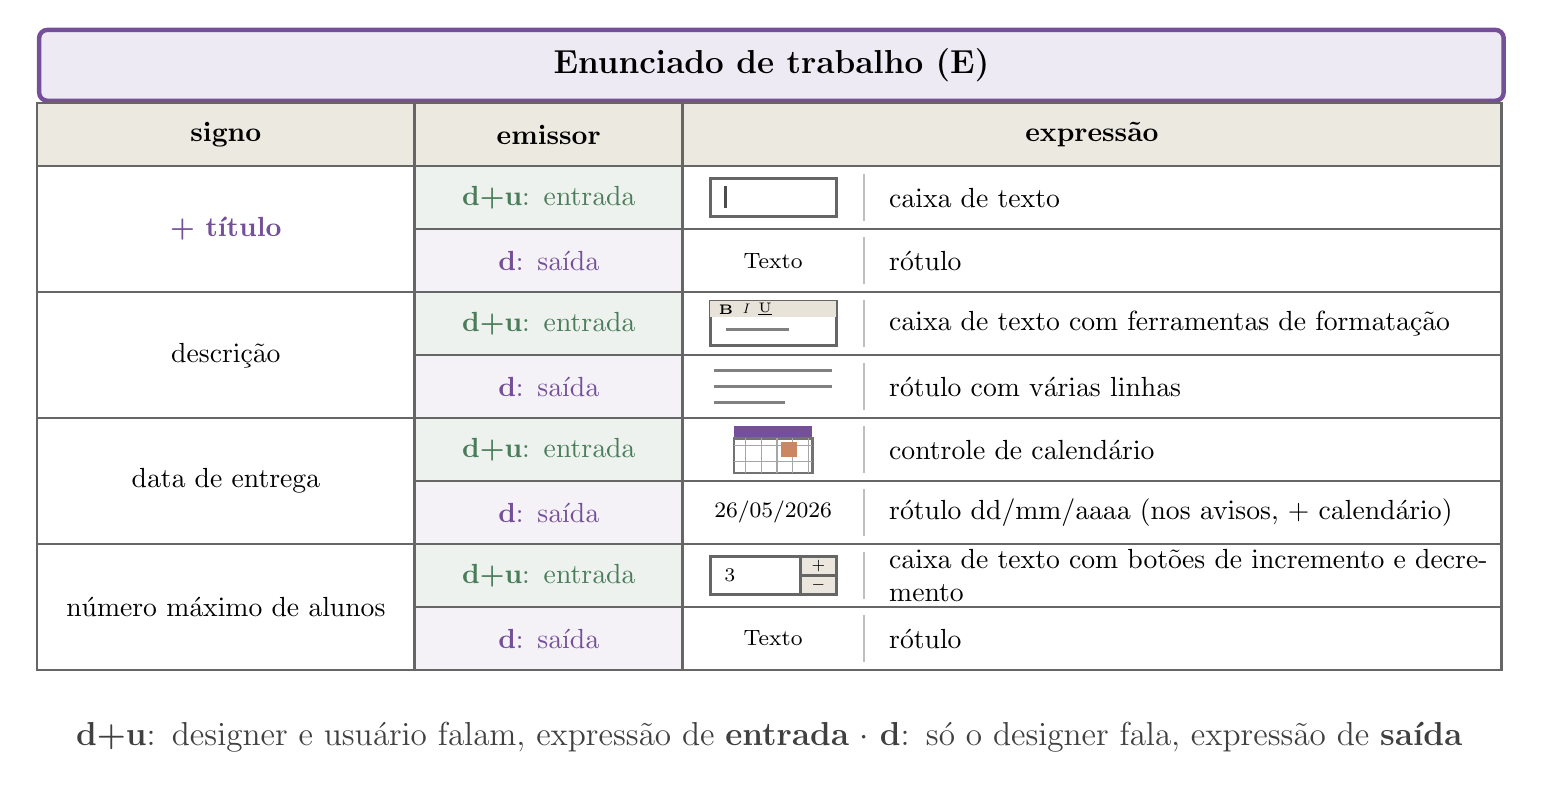
\begin{tikzpicture}[x=1cm,y=1cm]
\node[dbox, draw=dblue, fill=dblue!12, line width=1.6pt, minimum width=18.6cm, minimum height=0.9cm, font=\large\bfseries, anchor=south west, rounded corners=3pt] at (0,8.75) {Enunciado de trabalho (E)};
\draw[black!60, fill=dshade!55, line width=1pt] (0,7.95) rectangle (4.8,8.75);
\node[font=\normalsize\bfseries, text=black, text width=4.5cm, align=center] at (2.4,8.35) {signo};
\draw[black!60, fill=dshade!55, line width=1pt] (4.8,7.95) rectangle (8.2,8.75);
\node[font=\normalsize\bfseries, text=black, text width=3.1cm, align=center] at (6.5,8.35) {emissor};
\draw[black!60, fill=dshade!55, line width=1pt] (8.2,7.95) rectangle (18.6,8.75);
\node[font=\normalsize\bfseries, text=black, text width=10.1cm, align=center] at (13.4,8.35) {expressão};
\draw[black!60, fill=white, line width=1pt] (0,6.35) rectangle (4.8,7.95);
\node[font=\normalsize\bfseries, text=dblue, text width=4.5cm, align=center] at (2.4,7.15) {+ título};
\draw[black!60, fill=dgreen!10, line width=1pt] (4.8,7.15) rectangle (8.2,7.95);
\node[font=\normalsize, text=dgreen, text width=3.1cm, align=center] at (6.5,7.55) {\textbf{d+u}: entrada};
\draw[black!60, fill=white, line width=1pt] (8.2,7.15) rectangle (18.6,7.95);
\draw[black!25, line width=0.8pt] (10.5,7.25) -- (10.5,7.8500000000000005);
\draw[black!60, fill=white, line width=1pt] (8.549999999999999,7.31) rectangle (10.15,7.79);
\draw[black!70, line width=1pt] (8.75,7.41) -- (8.75,7.6899999999999995);
\node[font=\normalsize, anchor=west, text width=7.9cm, align=left] at (10.7,7.55) {caixa de texto};
\draw[black!60, fill=dblue!8, line width=1pt] (4.8,6.3500000000000005) rectangle (8.2,7.15);
\node[font=\normalsize, text=dblue, text width=3.1cm, align=center] at (6.5,6.75) {\textbf{d}: saída};
\draw[black!60, fill=white, line width=1pt] (8.2,6.3500000000000005) rectangle (18.6,7.15);
\draw[black!25, line width=0.8pt] (10.5,6.45) -- (10.5,7.050000000000001);
\node[font=\footnotesize] at (9.35,6.75) {Texto};
\node[font=\normalsize, anchor=west, text width=7.9cm, align=left] at (10.7,6.75) {rótulo};
\draw[black!60, fill=white, line width=1pt] (0,4.75) rectangle (4.8,6.35);
\node[font=\normalsize, text=black, text width=4.5cm, align=center] at (2.4,5.55) {descrição};
\draw[black!60, fill=dgreen!10, line width=1pt] (4.8,5.55) rectangle (8.2,6.35);
\node[font=\normalsize, text=dgreen, text width=3.1cm, align=center] at (6.5,5.95) {\textbf{d+u}: entrada};
\draw[black!60, fill=white, line width=1pt] (8.2,5.55) rectangle (18.6,6.35);
\draw[black!25, line width=0.8pt] (10.5,5.6499999999999995) -- (10.5,6.25);
\draw[black!60, fill=white, line width=1pt] (8.549999999999999,5.67) rectangle (10.15,6.23);
\fill[dshade!70] (8.549999999999999,6.03) rectangle (10.15,6.23);
\node[font=\tiny\bfseries] at (8.75,6.13) {B};\node[font=\tiny\itshape] at (9.0,6.13) {I};\node[font=\tiny] at (9.25,6.13) {\underline{U}};
\draw[black!50, line width=0.9pt] (8.75,5.87) -- (9.549999999999999,5.87);
\node[font=\normalsize, anchor=west, text width=7.9cm, align=left] at (10.7,5.95) {caixa de texto com ferramentas de formatação};
\draw[black!60, fill=dblue!8, line width=1pt] (4.8,4.75) rectangle (8.2,5.55);
\node[font=\normalsize, text=dblue, text width=3.1cm, align=center] at (6.5,5.15) {\textbf{d}: saída};
\draw[black!60, fill=white, line width=1pt] (8.2,4.75) rectangle (18.6,5.55);
\draw[black!25, line width=0.8pt] (10.5,4.85) -- (10.5,5.45);
\draw[black!50, line width=1.2pt] (8.6,5.3500000000000005) -- (10.1,5.3500000000000005);
\draw[black!50, line width=1.2pt] (8.6,5.15) -- (10.1,5.15);
\draw[black!50, line width=1.2pt] (8.6,4.95) -- (9.5,4.95);
\node[font=\normalsize, anchor=west, text width=7.9cm, align=left] at (10.7,5.15) {rótulo com várias linhas};
\draw[black!60, fill=white, line width=1pt] (0,3.15) rectangle (4.8,4.75);
\node[font=\normalsize, text=black, text width=4.5cm, align=center] at (2.4,3.95) {data de entrega};
\draw[black!60, fill=dgreen!10, line width=1pt] (4.8,3.95) rectangle (8.2,4.75);
\node[font=\normalsize, text=dgreen, text width=3.1cm, align=center] at (6.5,4.35) {\textbf{d+u}: entrada};
\draw[black!60, fill=white, line width=1pt] (8.2,3.95) rectangle (18.6,4.75);
\draw[black!25, line width=0.8pt] (10.5,4.05) -- (10.5,4.65);
\fill[dblue] (8.85,4.489999999999999) rectangle (9.85,4.6499999999999995);
\draw[black!55, line width=0.8pt, fill=white] (8.85,4.05) rectangle (9.85,4.489999999999999);
\draw[black!35, step=0.2, line width=0.5pt] (8.85,4.05) grid (9.85,4.489999999999999);
\fill[dorange!70] (9.45,4.25) rectangle (9.65,4.449999999999999);
\node[font=\normalsize, anchor=west, text width=7.9cm, align=left] at (10.7,4.35) {controle de calendário};
\draw[black!60, fill=dblue!8, line width=1pt] (4.8,3.1500000000000004) rectangle (8.2,3.95);
\node[font=\normalsize, text=dblue, text width=3.1cm, align=center] at (6.5,3.55) {\textbf{d}: saída};
\draw[black!60, fill=white, line width=1pt] (8.2,3.1500000000000004) rectangle (18.6,3.95);
\draw[black!25, line width=0.8pt] (10.5,3.2500000000000004) -- (10.5,3.85);
\node[font=\footnotesize] at (9.35,3.55) {26/05/2026};
\node[font=\normalsize, anchor=west, text width=7.9cm, align=left] at (10.7,3.55) {rótulo dd/mm/aaaa (nos avisos, + calendário)};
\draw[black!60, fill=white, line width=1pt] (0,1.5499999999999998) rectangle (4.8,3.15);
\node[font=\normalsize, text=black, text width=4.5cm, align=center] at (2.4,2.35) {número máximo de alunos};
\draw[black!60, fill=dgreen!10, line width=1pt] (4.8,2.3499999999999996) rectangle (8.2,3.15);
\node[font=\normalsize, text=dgreen, text width=3.1cm, align=center] at (6.5,2.75) {\textbf{d+u}: entrada};
\draw[black!60, fill=white, line width=1pt] (8.2,2.3499999999999996) rectangle (18.6,3.15);
\draw[black!25, line width=0.8pt] (10.5,2.4499999999999997) -- (10.5,3.05);
\draw[black!60, fill=white, line width=1pt] (8.549999999999999,2.51) rectangle (9.7,2.99);
\node[font=\scriptsize] at (8.799999999999999,2.75) {3};
\draw[black!60, fill=dshade!60, line width=1pt] (9.7,2.75) rectangle (10.15,2.99);
\draw[black!60, fill=dshade!60, line width=1pt] (9.7,2.51) rectangle (10.15,2.75);
\node[font=\tiny] at (9.924999999999999,2.87) {+};\node[font=\tiny] at (9.924999999999999,2.63) {$-$};
\node[font=\normalsize, anchor=west, text width=7.9cm, align=left] at (10.7,2.75) {caixa de texto com botões de incremento e decremento};
\draw[black!60, fill=dblue!8, line width=1pt] (4.8,1.5499999999999996) rectangle (8.2,2.3499999999999996);
\node[font=\normalsize, text=dblue, text width=3.1cm, align=center] at (6.5,1.95) {\textbf{d}: saída};
\draw[black!60, fill=white, line width=1pt] (8.2,1.5499999999999996) rectangle (18.6,2.3499999999999996);
\draw[black!25, line width=0.8pt] (10.5,1.6499999999999997) -- (10.5,2.2499999999999996);
\node[font=\footnotesize] at (9.35,1.95) {Texto};
\node[font=\normalsize, anchor=west, text width=7.9cm, align=left] at (10.7,1.95) {rótulo};
\node[font=\large, black!75, text width=18.6cm, align=center] at (9.3,0.7) {\textbf{d+u}: designer e usuário falam, expressão de \textbf{entrada} $\cdot$ \textbf{d}: só o designer fala, expressão de \textbf{saída}};
\end{tikzpicture}
\end{document}
